\begin{figure}[t]
\centering
\begin{minipage}[c]{0.64\textwidth}
\centering
\begin{subfigure}[t]{0.535\textwidth}
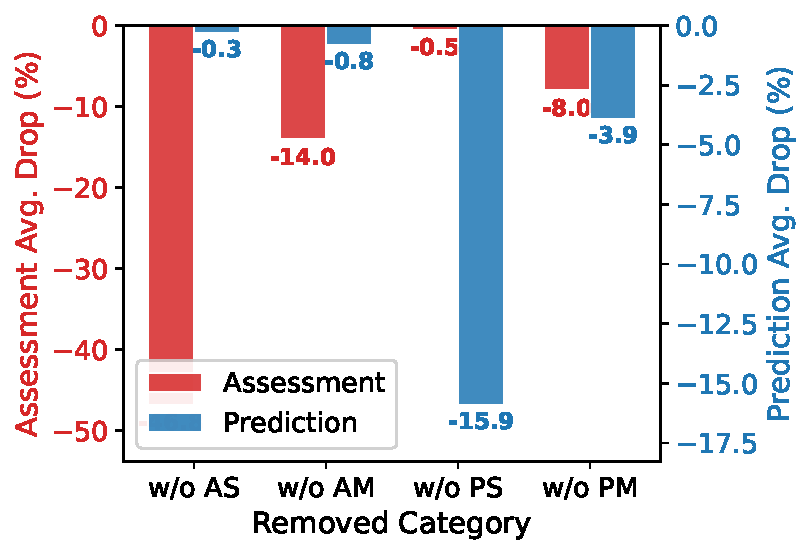
\includegraphics[width=\textwidth]{figures/placeholder_loco.pdf}
\caption{LOCO ablation.}
\end{subfigure}
\hfill
\begin{subfigure}[t]{0.45\textwidth}
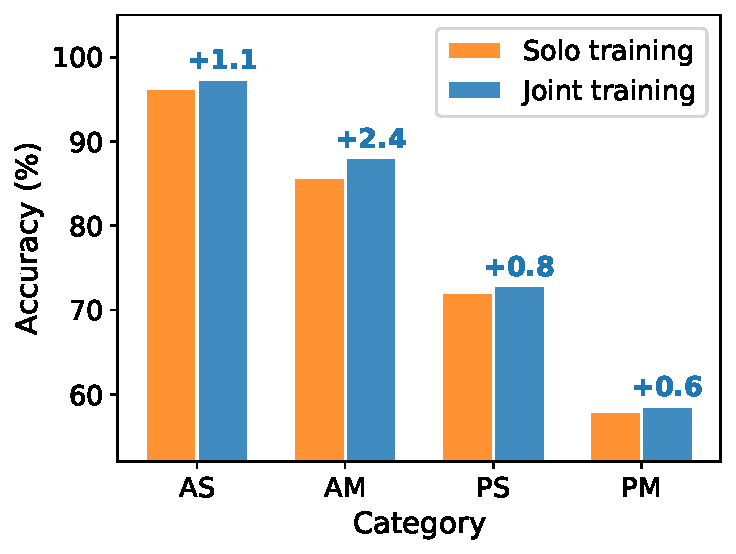
\includegraphics[width=\textwidth]{figures/placeholder_transfer.pdf}
\caption{Solo vs.\ joint training.}
\end{subfigure}
\caption{\textbf{Taxonomy dependency analysis.} (a) Each category is essential to its own tasks: removing AS causes the largest assessment drop ($-$46.8\%) and removing PS causes the largest prediction drop ($-$15.9\%). (b) Joint training across all four categories consistently outperforms solo training, indicating that the categories are complementary and mutually reinforcing.}
\label{fig:loco_analysis}
\end{minipage}
\hfill
\begin{minipage}[c]{0.35\textwidth}
\centering
\captionof{table}{Success rate on Test~A.}
\label{tab:sr}
\adjustbox{max width=\textwidth}{
\scriptsize
\begin{tabular}{lcc}
\toprule
\textbf{Model} & \textbf{SR} & \textbf{Acc.} \\
\midrule
\multicolumn{3}{l}{\textit{Language Models}} \\
Phi-3.5-mini & 4.8 & 2.7 \\
Mistral-7B & 41.6 & 21.2 \\
Gemma-2-9B & 51.8 & 28.3 \\
Llama-3.1-8B & 80.3 & 42.1 \\
Qwen2.5-7B & 99.9 & 51.6 \\
\midrule
\multicolumn{3}{l}{\textit{TS Language Models}} \\
TimeMQA-Qwen & 4.8 & 2.1 \\
TimeMQA-Mistral & 16.3 & 6.4 \\
TimeMQA-Llama & 25.4 & 10.4 \\
\midrule
\multicolumn{3}{l}{\textit{TS Reasoning Models}} \\
TimeOmni-1-7B & 98.8 & 51.3 \\
\midrule
\multicolumn{3}{l}{\textit{Ours}} \\
\rowcolor{yellow!15} \textbf{FinSTaR} & \first{100.0} & \first{78.9} \\
\bottomrule
\end{tabular}
}
\end{minipage}
\vspace{-10pt}
\end{figure}


\section{Analysis}
\label{sec:analysis}

\setlength{\columnsep}{1pt} 
\begin{wraptable}{r}{0.335\textwidth}
\vspace{-14pt}
\centering
\caption{Taxonomy of tasks.}
\label{tab:taxonomy_abbr}
\footnotesize
\adjustbox{max width=0.335\textwidth}{
\begin{tabular}{ll}
\toprule
\textbf{Abbr.} & \textbf{Category} \\
\midrule
\textbf{AS} & \textbf{A}ssessment-\textbf{S}ingle \\
\textbf{AM} & \textbf{A}ssessment-\textbf{M}ulti \\
\textbf{PS} & \textbf{P}rediction-\textbf{S}ingle \\
\textbf{PM} & \textbf{P}rediction-\textbf{M}ulti \\
\bottomrule
\end{tabular}
}
\vspace{-10pt}
\end{wraptable}
\textbf{Capability dependencies.}
We study how the \textit{four capability categories} (Table~\ref{tab:taxonomy_abbr}) interact during training via two complementary analyses on TimeOmni-1-7B on Test A.
First, we conduct a \textit{Leave-One-Category-Out} (LOCO) ablation: remove one category's tasks from training, retrain, and evaluate all ten tasks.
As shown in Figure~\ref{fig:loco_analysis}(a), each category is \textit{essential to its own tasks} --- removing AS causes the largest assessment drop and removing PS causes the largest prediction drop --- while removals do not catastrophically harm the other axis.
Second, Figure~\ref{fig:loco_analysis}(b) compares solo training (each category alone) with joint training (all four together): joint training \textit{consistently outperforms} solo training across all categories.
Together, these results show that the four categories are \textit{complementary and mutually reinforcing through joint training}, rather than redundant or interfering.
Full results are shown in Tables~\ref{tab:loco_full} and~\ref{tab:solo_joint}.


\textbf{Success rate.}
Table~\ref{tab:sr} reports the success rate (SR), the percentage of outputs containing a valid answer tag.
Most baselines fail to follow the required format: TimeMQA variants and Phi-3.5-mini achieve SR $<$ 25\%, rendering their accuracy unreliable.
In contrast, FinSTaR achieves 100\% SR, confirming that structured CoT supervision also teaches reliable output formatting.

\begin{table}[t]
\centering
\vspace{-32pt}
\begin{minipage}[t]{0.65\textwidth}
\centering
\caption{\textbf{Leave-One-Category-Out (LOCO) ablation study.} Each row removes one capability category from training and evaluates on all 10 tasks. Together with Table~\ref{tab:solo_joint}, the results reveal the dependencies among task categories and demonstrate the \textit{effectiveness of joint training across all four capabilities}.}
\label{tab:loco_full}
\vspace{5pt}
\adjustbox{max width=\textwidth}{
\begin{tabular}{l|cccc|cccccc|c}
\toprule
\multirow{2}{*}{ } & \multicolumn{4}{c|}{\textit{Assessment}} & \multicolumn{6}{c|}{\textit{Prediction}} & \multirow{2.5}{*}{\textbf{Avg.}} \\
\cmidrule(lr){2-5} \cmidrule(lr){6-11}
 & \textbf{Draw.} & \textbf{Vol.} & \textbf{Trend} & \textbf{Corr.} & \textbf{Event} & \textbf{S/R} & \textbf{DDR} & \textbf{V.F.} & \textbf{R.P.} & \textbf{P.C.} & \\
\midrule
\rowcolor{yellow!15} Full & \first{99.3} & \first{93.5} & \second{99.3} & \first{88.1} & \first{57.2} & \first{80.5} & 74.4 & \first{79.5} & \first{51.5} & \first{65.8} & \first{78.9} \\
\midrule
w/o AS & 43.2 & 32.2 & 29.2 & \second{88.0} & 56.8 & 79.8 & \first{75.3} & 78.8 & \first{51.5} & \second{65.4} & 60.0 \\
w/o AM & 98.8 & 92.3 & 99.2 & 33.4 & 53.9 & \second{80.4} & \second{75.2} & \second{78.9} & \first{51.5} & 64.4 & 72.8 \\
w/o PS & \second{99.2} & 90.6 & \first{99.4} & \second{88.0} & 47.7 & 48.1 & 47.4 & 55.1 & \first{51.5} & 64.1 & 69.1 \\
w/o PM & 98.9 & \second{92.3} & 67.5 & \first{88.1} & \second{57.1} & \second{80.4} & 74.8 & 76.6 & \second{47.8} & 49.2 & \second{73.3} \\
\bottomrule
\end{tabular}
}
\end{minipage}
\hfill
\begin{minipage}[t]{0.34\textwidth}
\centering
\captionof{table}{Solo vs.\ joint training.}
\label{tab:solo_joint}
\vspace{5pt}
\adjustbox{max width=\textwidth}{
\footnotesize
\begin{tabular}{c|l|cc|c}
\toprule
\textbf{Cat.} & \textbf{Task} & \textbf{Solo} & \textbf{Joint} & \textbf{$\Delta$} \\
\midrule
\multirow{3}{*}{AS} & Draw. & 98.8 & \cellcolor{yellow!15} \first{99.3} & \up{+0.5} \\
 & Vol. & 91.1 & \cellcolor{yellow!15} \first{93.5} & \up{+2.4} \\
 & Trend & 99.1 & \cellcolor{yellow!15} \first{99.3} & \up{+0.2} \\
\midrule
AM & Corr. & 85.7 & \cellcolor{yellow!15} \first{88.1} & \up{+2.4} \\
\midrule
\multirow{4}{*}{PS} & Event & 55.9 & \cellcolor{yellow!15} \first{57.2} & \up{+1.3} \\
 & S/R & 79.5 & \cellcolor{yellow!15} \first{80.5} & \up{+1.0} \\
 & DDR & \first{74.4} & \cellcolor{yellow!15} \first{74.4} & +0.0 \\
 & V.F. & 78.4 & \cellcolor{yellow!15} \first{79.5} & \up{+1.1} \\
\midrule
\multirow{2}{*}{PM} & R.P. &\first{51.5} & \cellcolor{yellow!15} \first{51.5} & +0.0 \\
 & P.C. & 64.5 & \cellcolor{yellow!15} \first{65.8} & \up{+1.3} \\
\bottomrule
\end{tabular}
}
\end{minipage}

\vspace{18pt}

% --- Forecasting baselines ---
\captionof{table}{\textbf{Forecasting baselines on prediction.} Values are (Test~A, Test~B, Test~C). FinSTaR outperforms forecasting baselines, with the largest gains on tasks requiring scenario reasoning.}
\label{tab:forecast_vs_reasoning}
\vspace{3pt}
\adjustbox{max width=\textwidth}{
\footnotesize
\begin{tabular}{l|cccccc|c}
\toprule
\textbf{Method} & \textbf{Event} & \textbf{S/R} & \textbf{DDR} & \textbf{V.F.} & \textbf{R.P.} & \textbf{P.C.} & \textbf{Avg.} \\
\midrule
\midrule
\multicolumn{8}{l}{\textit{Statistical Forecasting}} \\
\midrule
Last Value & (42.7, 44.5, 46.4) & (61.7, 62.1, 59.6) & (49.9, 51.2, 49.3) & (48.0, 53.6, 51.9) & (48.5, 49.9, 47.0) & (50.3, 48.3, 49.1) & (50.2, 51.6, 50.5) \\
ETS & (49.2, 52.0, 50.3) & (62.1, 59.5, 58.9) & (46.3, 47.6, 49.9) & (48.0, 53.6, 51.9) & (49.5, \second{53.9}, 50.2) & (54.6, 56.5, 52.3) & (51.6, 53.8, 52.2) \\
MA & (51.2, 52.7, 52.1) & (60.1, 57.2, 57.8) & (45.1, 46.1, 46.3) & (50.6, 56.8, 53.9) & (50.8, 53.2, 51.3) & (\second{59.0}, \second{57.6}, \second{56.5}) & (52.8, 53.9, 53.0) \\
Momentum & (49.5, 47.2, 50.4) & (68.9, 68.8, 68.4) & (57.1, 55.6, 57.6) & (48.0, 53.6, 51.9) & (49.7, 45.9, 49.0) & (50.5, 49.5, 52.3) & (53.9, 53.4, 54.9) \\
Drift & (52.9, 50.7, 50.4) & (71.0, 72.5, 68.1) & (\second{63.5}, \second{66.0}, \second{64.1}) & (48.0, 53.6, 51.9) & (48.4, 47.8, 50.4) & (50.3, 48.3, 49.1) & (55.7, 56.5, 55.7) \\
\midrule
\midrule
\multicolumn{8}{l}{\textit{DL Forecasting}} \\
\midrule
TFT & (52.8, 53.0, 50.6) & (61.6, 60.2, 58.1) & (36.3, 38.9, 39.9) & (48.0, 53.7, 51.9) & (50.4, 49.2, \first{54.3}) & (52.2, 50.9, 50.4) & (50.2, 51.0, 50.9) \\
DeepAR & (49.1, 53.1, 51.2) & (64.0, 61.4, 60.6) & (50.4, 50.3, 51.0) & (48.2, 54.2, 52.0) & (48.4, 53.7, 49.9) & (56.4, 55.9, 56.2) & (52.8, 54.8, 53.5) \\
DLinear & (47.9, 48.7, 52.0) & (63.8, 62.1, 58.5) & (64.9, \second{66.9}, 63.0) & (58.2, 55.3, 57.7) & (46.4, 52.5, 50.2) & (55.0, 56.8, 54.8) & (56.0, \second{57.0}, 56.0) \\
TiDE & (\second{54.1}, \second{54.4}, \second{53.0}) & (57.4, 54.6, 56.7) & (58.1, 57.2, 56.7) & (\second{58.9}, 55.6, \second{58.0}) & (50.5, \first{54.1}, 50.3) & (56.2, \second{57.5}, \second{57.0}) & (55.9, 55.6, 55.3) \\
PatchTST & (48.6, 49.2, 49.6) & (\second{80.4}, \second{79.7}, \second{79.1}) & (49.3, 48.7, 49.1) & (69.5, \second{64.6}, 68.9) & (48.2, 48.6, 48.5) & (48.4, 44.9, 47.7) & (\second{57.4}, 56.0, \second{57.1}) \\
Chronos-1 & (53.4, \second{54.9}, 48.9) & (69.4, 71.0, 66.5) & (50.2, 53.9, 50.1) & (47.9, 54.2, 52.0) & (50.1, 48.0, 49.8) & (53.0, 51.0, 53.0) & (54.0, 55.5, 53.4) \\
Chronos-2 & (53.2, 53.0, 51.1) & (67.9, 69.5, 64.4) & (45.3, 47.0, 46.3) & (48.0, 53.6, 51.9) & (\second{51.4}, 49.1, \second{52.4}) & (53.2, 48.2, 51.3) & (53.2, 53.4, 52.9) \\
\midrule
\midrule
\multicolumn{8}{l}{\textit{Financial TSRM (Ours)}} \\
\midrule
\rowcolor{yellow!15} \textbf{FinSTaR} & (\first{57.2}, \first{55.6}, \first{53.5}) & (\first{80.5}, \first{80.0}, \first{79.5}) & (\first{74.4}, \first{75.0}, \first{72.9}) & (\first{79.5}, \first{77.3}, \first{78.8}) & (\first{51.5}, 50.1, 53.0) & (\first{65.8}, \first{64.3}, \first{64.6}) & (\first{68.2}, \first{67.0}, \first{67.0}) \\
\bottomrule
\end{tabular}
}
% \vspace{-14pt}
\end{table}

\textbf{Prediction tasks: TSRM vs.\ TS forecasting models.}
While TSRMs can handle both assessment and prediction through reasoning, traditional TS forecasting models can also solve prediction tasks without reasoning, via a \textit{forecast-then-classify} pipeline (predict future prices numerically, then convert to classification labels).
We compare FinSTaR against such forecasting models: statistical methods (Last Value, MA, ETS, Drift, Momentum) and DL models (DLinear~\cite{dlinear}, Chronos-1/2~\cite{chronos2024}, DeepAR~\cite{deepar}, PatchTST~\cite{patchtst}, TFT~\cite{tft}, TiDE~\cite{tide}).
As shown in Table~\ref{tab:forecast_vs_reasoning},
FinSTaR outperforms the forecasting models on prediction tasks.
Details of forecasting models are discussed in Appendix~\ref{app:forecast_protocol}.
%The advantage is most pronounced on Drawdown Recovery and Volatility Forecast, where scenario reasoning captures volatility clustering and mean-reversion dynamics that numerical extrapolation misses.

\textbf{Backbone sensitivity.}
Table~\ref{tab:backbone} compares the effect of CoT across two backbones: TimeOmni-1-7B (trained with TS reasoning SFT + RL) and Qwen2.5-7B (general-purpose LLM without TS-specific training).\footnote{Both Qwen2.5-7B rows (w/o CoT and w/ CoT) are fine-tuned on the same FinTSR-Bench data via LoRA, serving as SFT baselines that isolate the effect of TS reasoning pre-training from our CoT strategies.}
CoT improves assessment accuracy for both backbones, since Compute-in-CoT involves explicit arithmetic that even general-purpose LLMs can perform.
However, for prediction tasks, CoT improves TimeOmni-1 (+11.3\%) but \textit{hurts} Qwen ($-$5.0\%).
We attribute this to the fact that Scenario-Aware CoT requires reasoning about price dynamics, which demands prior TS reasoning ability.
Without TS reasoning training, the general-purpose LLM generates plausible-sounding but ungrounded scenarios, introducing noise rather than useful reasoning signal.
This suggests that \textit{Scenario-Aware CoT is effective only when the backbone already possesses TS reasoning ability}, highlighting the synergy between TS reasoning pre-training and structured CoT supervision.

% \textbf{Training dynamics.}
% We observe that assessment tasks converge by Epoch~1--2, while prediction tasks improve until Epoch~3--4 (see Figure~\ref{fig:epoch} in Appendix~\ref{app:epoch}).

\textbf{Effect of training set size.} 
We evaluate FinSTaR’s performance with a reduced training data size.
%(350, 875, 1750, and 3500 samples per task).
As shown in Table~\ref{tab:data_eff_full}, FinSTaR already achieves 71.7\% overall accuracy
with only 350 samples/task (10\% of full).
Performance improves to 74.7\% at 875 and 75.2\% at 1750 samples, with diminishing returns beyond that.
This indicates that our Compute-in-CoT and Scenario-Aware CoT strategies are \textit{data-efficient}, requiring relatively few examples to learn the underlying reasoning patterns.

\begin{table}[t]
\vspace{-25pt}
\centering
\caption{\textbf{Backbone sensitivity.} Scenario-Aware CoT improves prediction only with a TS reasoning-trained backbone (TimeOmni-1, +11.3\%), while it hurts the general-purpose LLM (Qwen, $-$5.0\%), suggesting that \textit{prior TS reasoning ability is necessary} for effective scenario-based reasoning.}
\label{tab:backbone}
\vspace{5pt}
\adjustbox{max width=0.95\textwidth}{
\begin{tabular}{c|l|cc|c}
\toprule
\textbf{Backbone} & \textbf{Config} & \textbf{Assessment Avg.} & \textbf{Prediction Avg.} & \textbf{Overall} \\
\midrule
\multirow{3.5}{*}{\shortstack{Qwen2.5-7B\\(w/o TS Reasoning SFT)}} & w/o CoT & 57.0 & \first{56.1} & 56.4 \\
 & \cellcolor{yellow!15}  w/ CoT & \cellcolor{yellow!15}  \first{67.7} & \cellcolor{yellow!15}  51.1 & \cellcolor{yellow!15}  \first{57.8} \\
 \cmidrule(lr){2-5}
 & $\Delta$ & \up{+10.7} & $-$5.0 & \up{+1.3} \\
\midrule
\multirow{3.5}{*}{\shortstack{TimeOmni-1-7B\\(w/ TS Reasoning SFT)}} & w/o CoT & 54.3 & 56.9 & 55.9 \\
 & \cellcolor{yellow!15}   w/ CoT & \cellcolor{yellow!15}  \first{95.0} & \cellcolor{yellow!15}  \first{68.2} & \cellcolor{yellow!15}  \first{78.9} \\
  \cmidrule(lr){2-5}
 & $\Delta$ & \up{+40.7} & \up{+11.3} & \up{+23.1} \\
\bottomrule
\end{tabular}
}
\vspace{-12pt}
\end{table}

\begin{table}[t]
\centering
\caption{\textbf{Effect of training set size.} FinSTaR performance with 350, 875, 1750, and 3500 training samples per task. With only 10\% of the full data (350 samples/task), FinSTaR already achieves 71.7\%, indicating that \textit{structured CoT strategies are sample-efficient.}}
\vspace{5pt}
\label{tab:data_eff_full}
\adjustbox{max width=\textwidth}{
\begin{tabular}{l|l|cccc|cccccc|c}
\toprule
 \multirow{2.5}{*}{\textbf{Method}} &\multirow{2.5}{*}{\textbf{\# Samples}} & \multicolumn{4}{c|}{\textit{Assessment}} & \multicolumn{6}{c|}{\textit{Prediction}} & \multirow{2.5}{*}{\textbf{Avg.}} \\
\cmidrule(lr){3-6} \cmidrule(lr){7-12}
& & \textbf{Draw.} & \textbf{Vol.} & \textbf{Trend} & \textbf{Corr.} & \textbf{Event} & \textbf{S/R} & \textbf{DDR} & \textbf{V.F.} & \textbf{R.P.} & \textbf{P.C.} & \\
\midrule
\rowcolor{gray!15} TimeOmni-1-7B & 3500 (100\%) &  75.7 & 35.6 & 50.5 & 31.5 & 49.1 & 54.1 & 59.3 & 58.2 & 50.7 & 48.4 & 51.3 \\
\rowcolor{gray!15}Qwen2.5-7B (w/o CoT) & 3500 (100\%) &  77.5 & 40.4 & 75.2 & 34.7 & 53.0 & 53.7 & 67.1 & 60.6 & 50.7 & 51.3 & 56.4 \\
\rowcolor{gray!15}Qwen2.5-7B (w/ CoT)& 3500 (100\%) & 96.4 & 46.6 & 92.3 & 35.4 & 47.6 & 51.1 & 57.2 & 48.7 & 47.3 & 55.0 & 57.8 \\
\midrule
\multirow{4}{*}{\textbf{FinSTaR}} & 350 (10\%) &  98.1 & 80.4 & 98.0 & 71.6 & 53.9 & 54.8 & 70.6 & 73.9 & 51.4 & 63.8 & 71.7 \\
& 875 (25\%)& 98.0 & 87.3 & 99.0 & 83.1 & 57.4 & 53.9 & 73.6 & 78.2 & 51.5 & 64.5 & 74.7 \\
& 1750 (50\%)& 99.1 & 90.0 & 82.2 & 85.5 & 54.5 & 70.9 & 74.7 & 78.7 & 51.5 & 65.0 & 75.2 \\
& 3500  (100\%)& 99.3 & 93.5 & 99.3 & 88.1 & 57.2 & 80.5 & 74.4 & 79.5 & 51.5 & 65.8 & 78.9 \\
\bottomrule
\end{tabular}
}
\vspace{-11pt}
\end{table}

\textbf{CoT quality verification.}
We verify that FinSTaR generates meaningful reasoning rather than template copies along four dimensions, with details provided in Appendix~\ref{app:tasks}:
\setlist[itemize]{leftmargin=0.3cm, itemsep=0.2pt, parsep=0pt, topsep=1pt}
\begin{itemize}
\item \textbf{Format compliance.} Over 99\% of outputs contain valid \texttt{<think>...<answer>} structure.
\item \textbf{Arithmetic faithfulness.} Since each assessment label is uniquely determined by a numerical computation, the near-perfect accuracy ($>$93\%) implies faithful intermediate reasoning. Manual inspection confirms that computed values align with ground truth.
\item \textbf{Scenario diversity.} Across 100 sampled prediction outputs, 85+ unique scenario descriptions per task confirm that the model \textit{generates varied reasoning, not memorized templates}.
While scenario templates are defined per (task, answer) pair during training, this does not constitute label leakage: the model generates all three scenarios \textit{before} selecting an answer, and the template serves as a reasoning scaffold rather than an answer key.
\item \textbf{Output length.} Prediction CoT averages ${\sim}249$ tokens, approximately 2.4$\times$ longer than assessment CoT (${\sim}104$ tokens), reflecting the additional scenario analysis steps.
%\item \textbf{Prediction calibration.} FinSTaR achieves an average Brier score of 0.319 on the six prediction tasks, outperforming Qwen (0.497) and TimeOmni-1 (0.467) on all tasks, demonstrating that structured CoT supervision improves not only accuracy but also \textit{prediction reliability} (Appendix~\ref{app:calibration}).
\end{itemize}


% \textbf{Qualitative comparison.}
% Figure~\ref{fig:qualitative} shows two representative examples where only FinSTaR answers correctly while both baselines fail.
% In the Event Response example, Qwen and TimeOmni both default to mean-reversion reasoning, ignoring the strong z-score (+4.52) and pre-event downward trend that suggest persistence. FinSTaR's Scenario-Aware CoT explicitly evaluates base/adverse/favorable outcomes and correctly identifies persistence.
% In the Volatility Regime example, Qwen computes nothing and guesses; TimeOmni attempts calculation but makes errors, arriving at a ratio of ${\sim}1$ (Normal). FinSTaR precisely computes the ratio as 2.38 and correctly classifies High volatility.

